\documentclass[tikz, border = 5pt]{standalone}
\usepackage{tikz}

\usetikzlibrary{arrows.meta}
\usetikzlibrary{shapes.geometric}


\begin{document}

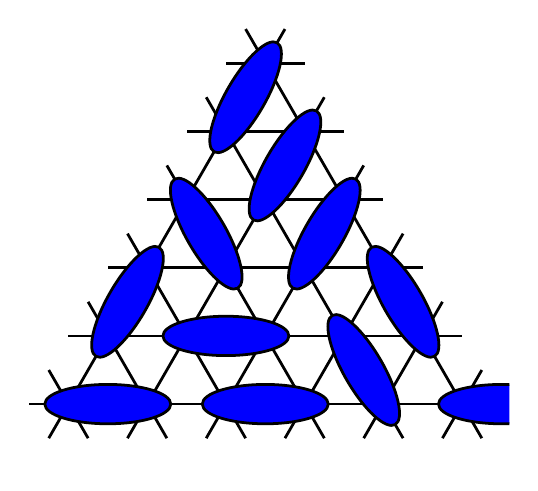
\begin{tikzpicture}[scale = 1.0]

	% model Parameters
	\def \base{6}	% number of sites in base
	\def \a{1}	% lattice paramters

	% artistic parameters
	\def \lw{1pt}
	\def \ellength{0.8} % in units of a!
	\def \elheigth{0.25} % in units of a!
	\def \elfillcolor{blue}
	\def \ellinecolor{black}
	\def \ellinewidth{1}

	% get physical coordiantes of points from i and j
	\newcommand{\getpoint}[2]{%
    		\pgfmathsetmacro{\X}{\a*(#1-0.5*#2)}%
    		\pgfmathsetmacro{\Y}{\a*#2*sqrt(3)/2}%
	}


	% define arrow 
	% parmeters: coeff t_1/a = x, coeff t_2/a = -x/2 + y*sqrt(3)/2, length, rotation angle in degree (0 is positive x-direction)
	% optional parameters: color, line width

	\NewDocumentCommand{\drawarrow}{m m m m O{black} O{0.4pt}}{
		\getpoint{#1}{#2}
		\draw[-{Stealth}, line width = #6, draw = #5]({\X - #3*cos(#4)/3}, {\Y - #3*sin(#4)/3}) -- ({\X + 2*#3*cos(#4)/3}, {\Y + 2*#3*sin(#4)/3});
	}

	
	% define ellipse, used for RVB state illustrations
	% parameters: t_1 coeff first point, t_2 coeff first point, t_1 coefff second point, t_2 coeff second point

	\NewDocumentCommand{\drawellipse}{m m m m}{

		\pgfmathsetmacro{\X}{\a*(#1+#3-(#2+#4)/2)/2}
		\pgfmathsetmacro{\Y}{\a*sqrt(3)*(#2+#4)/4}
		\pgfmathsetmacro{\rot}{\a*atan(sqrt(3)*(#4-#2)/(2*(#3-#1-#4/2+#2/2)))}

		\draw[draw=\ellinecolor, fill=\elfillcolor, line width = \ellinewidth, rotate around={\rot: (\X, \Y)}] (\X, \Y) ellipse[x radius = \a*\ellength, y radius = \a*\elheigth];
	}


	% Create lattice points 
	\foreach \i in {1,...,\base}{
		\foreach \j in {1,...,\i}{
			\getpoint{\i}{\j}
			\coordinate (P-\i-\j) at (\X, \Y);
		}
	}


	% Draw nearest neighbour links
	\foreach \i in {1,...,\base}{
		\foreach \j in {1,...,\i}{
				
			% to right and top right:
			\ifnum \i < \base 
				\draw[line width = \lw] (P-\i-\j) -- (P-\the\numexpr\i+1\relax-\j);
				\draw[line width = \lw] (P-\i-\j) -- (P-\the\numexpr\i+1\relax-\the\numexpr\j+1\relax);
			\fi

			% to top left 
			\ifnum \j < \i
				\draw[line width = \lw] (P-\i-\j) -- (P-\i-\the\numexpr\j+1\relax);
			\fi	
		}
	}

	% Draw half-length nearest neighbour lines outwards from outermost sites

	% Bottom edge
	\foreach \i in {1,...,\base}{
		\draw[line width = \lw] (P-\i-1) -- ++ (0.25*\a ,{-sqrt(3)/4*\a});
		\draw[line width = \lw] (P-\i-1) -- ++ (-0.25*\a ,{-sqrt(3)/4*\a});
	}
	
	% Right edge
	\foreach \j in {1,...,\base}{
		\draw[line width = \lw] (P-\base-\j) -- ++ (0.5*\a, 0);
		\draw[line width = \lw] (P-\base-\j) -- ++ (0.25*\a, {sqrt(3)*\a/4});
	}

	% Left edge
	\foreach \i in {1,...,\base}{
		\draw[line width = \lw] (P-\i-\i) -- ++ (-0.5*\a, 0);
		\draw[line width = \lw](P-\i-\i) -- ++ (-0.25*\a, {sqrt(3)*\a/4});
	}
	
	% draw ellipses
	\drawellipse{1}{1}{2}{1}
	\drawellipse{3}{2}{4}{2}
	\drawellipse{2}{2}{3}{3}
	\drawellipse{3}{1}{4}{1}
	\drawellipse{4}{3}{4}{4}
	\drawellipse{5}{5}{6}{6}
	\drawellipse{5}{4}{6}{5}
	\drawellipse{5}{3}{6}{4}	
	\drawellipse{5}{1}{5}{2}
	\drawellipse{6}{2}{6}{3}
	
	% draw clipped ellipse in the bottom right corner:
	\begin{scope}
		\clip ({\a*(6 - 1.25*\ellength)}, {\a*sqrt(3)/2-\elheigth-\ellinewidth/2}) rectangle ({\a*6.1}, {\a*sqrt(3)/2+\elheigth+\ellinewidth/2});
		\drawellipse{6}{1}{7}{1}	
	\end{scope}



\end{tikzpicture}

\end{document}
	
